\section{Further W+MET models with possible cross-section enhancements} 

%Contributed by Yang Bai

As pointed out in Ref.~\cite{Bell:2015sza}, the mono-$W$ signature can probe the iso-spin violating interactions of dark matter with quarks. The relevant operators after the electroweak symmetry breaking is 
%
\begin{equation}
\frac{1}{\Lambda^2}\overline{\chi} \gamma_\mu \chi \left( \overline{u}_L \gamma^\mu u_L + \xi \bar{d}_L \gamma^\mu d_L \right) \,.
\end{equation}
%
Here, we only keep the left-handed quarks because the right-handed quarks do not radiate a $W$-gauge boson from the weak interaction. As the LHC constraints the cutoff to higher values, it is also important to know the corresponding operators before the electroweak symmetry. At the dimension-six level, the following operator
%
\begin{equation}
\frac{c_6}{\Lambda^2}\overline{\chi} \gamma_\mu \chi \,\overline{Q}_L \gamma^\mu Q_L 
\end{equation}
%
conserves iso-spin and provides us $\xi=1$~\cite{1503.07874}. At the dimension-eight level, new operators appear to induce iso-spin violation and can be
%
\begin{equation}
\frac{c^d_8}{\Lambda^4}\overline{\chi} \gamma_\mu \chi \,(H\overline{Q}_L) \gamma^\mu (Q_L H^\dagger) 
+ \frac{c^u_8}{\Lambda^4}\overline{\chi} \gamma_\mu \chi \,(\tilde{H}\overline{Q}_L) \gamma^\mu (Q_L \tilde{H}^\dagger)  \,.
\end{equation}
% 
After inputting the vacuum expectation value of the Higgs field, we have 
\begin{equation}
\xi = \frac{c_6 \,+\, c_8^d\,v_{\rm EW}^2/2\Lambda^2}{c_6 \,+\, c_8^u \,v_{\rm EW}^2/2\Lambda^2} \,.
\end{equation}
% 
For a nonzero $c_6$ and $v_{\rm EW} \ll \Lambda$, the iso-spin violation effects are suppressed. On the other hand, the values of $c_6$, $c^d_8$ and $c^u_8$ depend on the UV-models. 

There is one possible UV-model to obtain a zero value for $c_6$ and non-zero values for $c^d_8$ and $c^u_8$. One can have the dark matter and the SM Higgs field charged under a new $U(1)^\prime$. There is a small mass mixing between SM $Z$-boson and the new $Z^\prime$ with a mixing angle of ${\cal O}(v_{\rm EW}^2/M^2_{Z^\prime})$. After integrating out $Z^\prime$, one has different effective dark matter couplings to $u_L$ and $d_L$ fields, which are proportional to their couplings to the $Z$ boson. For this model, we have $c_6=0$ and 
 %
\begin{equation}
\xi = \frac{-\frac{1}{2} + \frac{1}{3} \sin^2{\theta_W} }{ \frac{1}{2} - \frac{2}{3} \sin^2{\theta_W}} \approx  -2.7 
\end{equation}
%
and order of unity. 

\section{Simplified model corresponding to dimension-5 EFT operator}

% +++++++++++++++++++++++++++++++++++++++++++++++++++++++++++++++++++++++++++++++++++++
%   Linda 11/5/15
% +++++++++++++++++++++++++++++++++++++++++++++++++++++++++++++++++++++++++++++++++++++

As an example of a simplified model corresponding to the dimension-5 EFT operator 
described in Section~\ref{sec:EFT_models_with_direct_DM_boson_couplings}, 
we consider a Higgs portal with a scalar mediator. Models of this kind
are among the most concise versions of simplified models that produce 
couplings of Dark Matter to pairs of gauge-bosons.  Scalar fields may couple directly to pairs of electroweak gauge bosons, 
but must carry part of the electroweak vev.  One may thus consider a simple model where Dark Matter couples to a a scalar 
singlet mediator, which mixes with the fields in the Higgs sector.
\begin{equation}
L\subset m_s S^2 + \lambda S^2H^2 +\lambda^{'} S H^2 + y S \chi \overline{\chi}
\end{equation}
Where H is a field in the Higgs sector that contains part of the electroweak vev, 
S is a heavy scalar singlet and $\chi$ is a Dark Matter field. 
There is then an S channel diagram where DM pairs couple to the singlet field S, 
which then mixes with a Higgs-sector field, and couples to W and Z bosons. 
This diagram contains 2 insertions of EW symmetry breaking fields, 
corresponding in form to the effective dimension-5 operator in the previous section.   

\section{Tabulated cross-sections}

\subsection{photon+MET signal, s-channel vector mediator model}

\subsection{Higgs+MET signal, vector mediator model}

Figure~\ref{fig:zprimeXS} shows the cross sections in this vector mediator model in the $m_{med}$ 
vs $m_{DM}$ plane. The tabulated values can be found in Table~\ref{tab:zprimeXS}

\begin{figure}[hbpt!]
	\begin{center}
		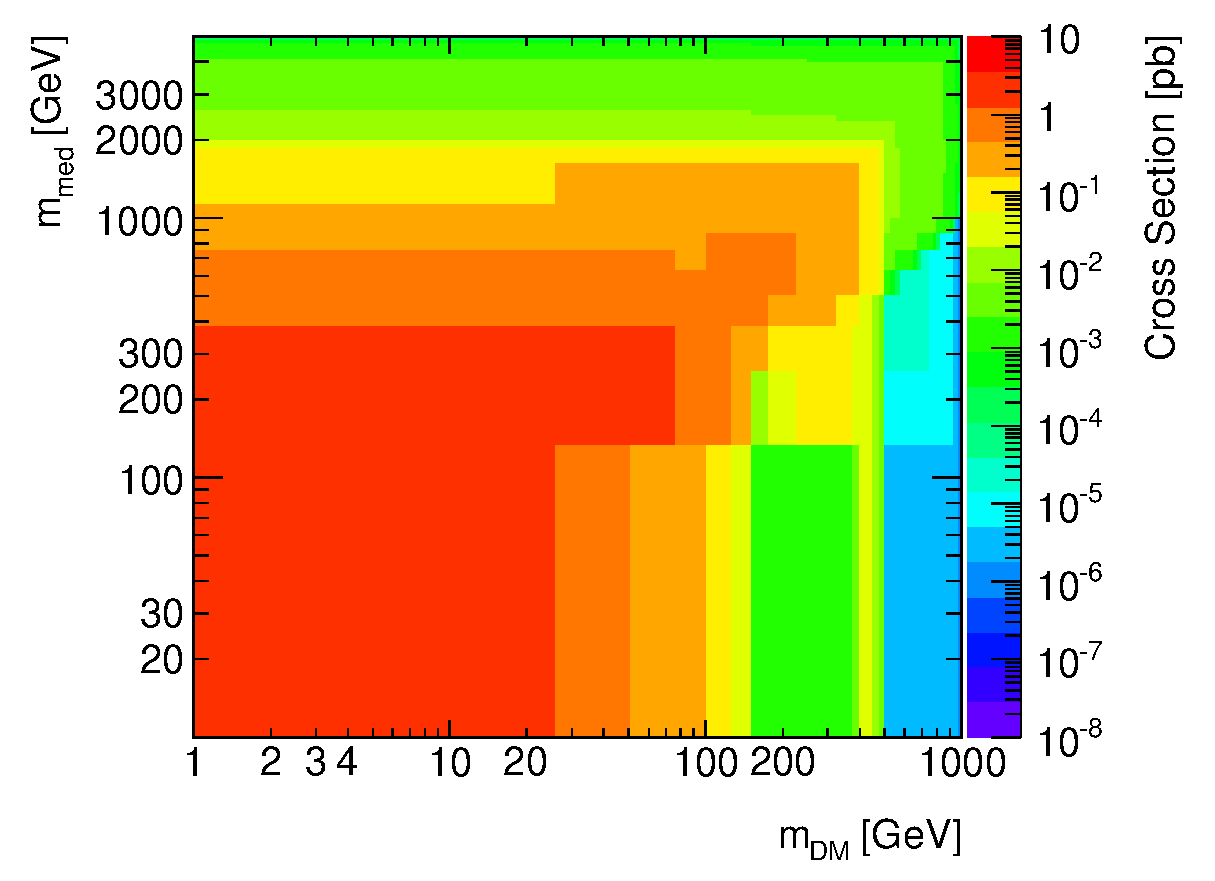
\includegraphics[width=0.9\linewidth]{figures/EW/monoH/zprime_cross_section_new}
		\caption{ Cross section of the $pp \rightarrow H\chi\bar{\chi}$ process 
			in units of pico-barn for the vector mediator model. 
			\label{fig:zprimeXS}}
	\end{center}
\end{figure}


\begin{table}
	\centering
	\begin{tabular}{ccc}
		$m_{DM}$ [GeV] & $m_{med}$ [GeV] & $\sigma_{pp\rightarrow h\chi\bar{\chi}}$ [pb] \\ \hline
		1 & 10 & 0.0003835 \\
		1 & 20 & 0.0003177 \\
		1 & 50 & 0.0001467 \\
		1 & 100 & 0.0001065 \\
		1 & 200 & 6.867e-05 \\
		1 & 300 & 7.388e-05 \\
		1 & 500 & 7.858e-05 \\
		1 & 1000 & 4.327e-05 \\
		1 & 2000 & 4.018e-05 \\
		1 & 5000 & 3.336e-05 \\ \hline
		10 & 10 & 3.603e-06 \\
		10 & 15 & 1.477e-05 \\
		10 & 50 & 0.0001547 \\
		10 & 100 & 0.0001104 \\
		10 & 5000 & 4.5e-05 \\ \hline
		50 & 10 & 1.401e-07 \\
		50 & 50 & 2.099e-07 \\
		50 & 95 & 2.813e-05 \\
		50 & 200 & 4.82e-05 \\
		50 & 300 & 7.485e-05 \\
		50 & 5000 & 3.384e-05 \\ \hline
		150 & 10 & 4.833e-09 \\
		150 & 295 & 3.65e-08 \\
		150 & 500 & 6.463e-07 \\
		150 & 5000 & 2.407e-08 \\ \hline
		500 & 10 & 8.672e-12 \\
		500 & 500 & 1.157e-11 \\
		500 & 995 & 5.254e-10 \\
		500 & 2000 & 7.138e-10 \\
		500 & 5000 & 5.87e-10 \\ \hline
		1000 & 10 & 5.946e-14 \\
		1000 & 1000 & 1.546e-13 \\
		1000 & 1995 & 8.316e-12 \\
		1000 & 5000 & 2.112e-11 \\ \hline
	\end{tabular}
	\caption{ Cross section of the $pp \rightarrow h\chi\bar{\chi}$ process 
		in units of pico-barn for the vector mediator model. 
		\label{tab:zprimeXS}}
\end{table}

\subsection{Higgs+MET signal, scalar mediator model}

Figure~\ref{fig:scalarXS} shows the cross sections of the $pp \rightarrow H\chi\bar{\chi}$ process 
in this vector mediator model in the $m_{med}$ 
vs $m_{DM}$ plane. The tabulated values can be found in Table~\ref{tab:scalarXS}

\begin{figure}[hbpt!]
	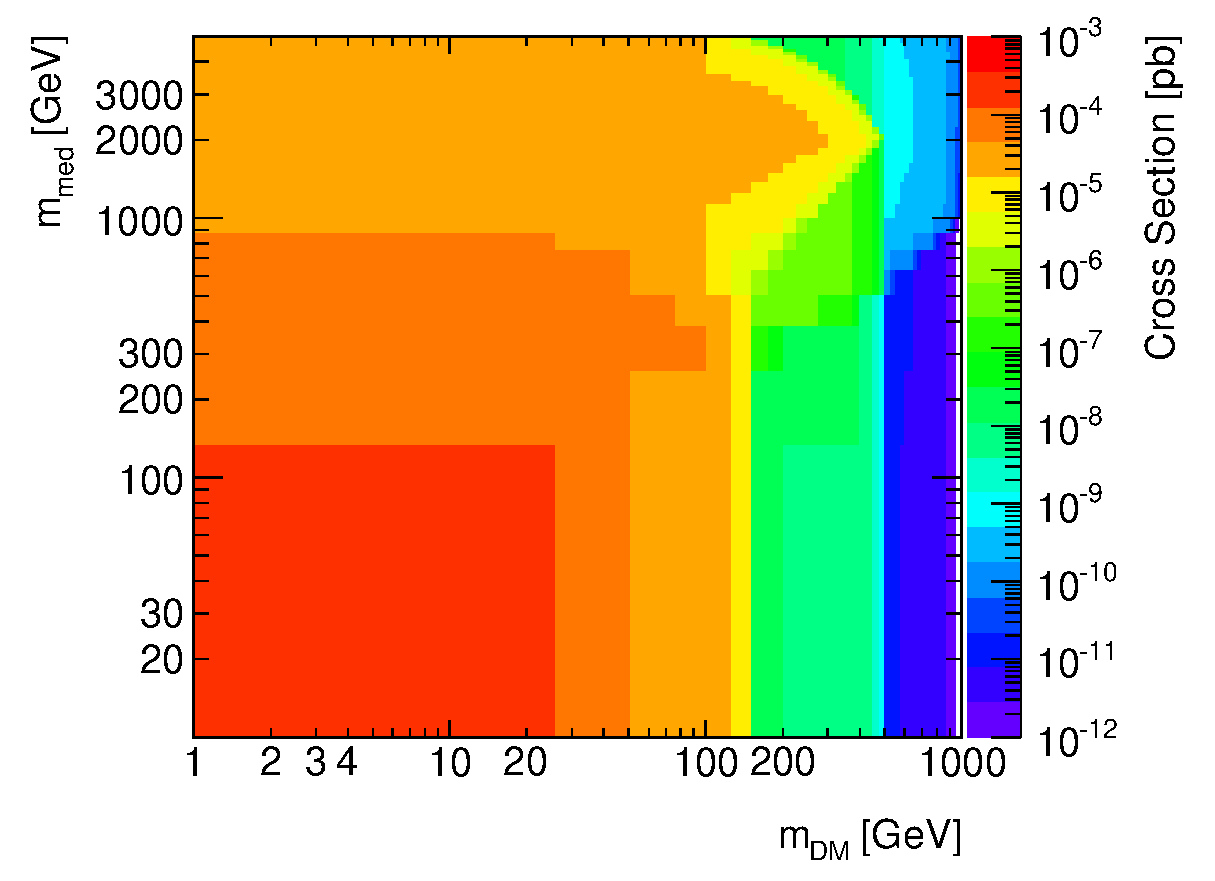
\includegraphics[width=0.8\linewidth]{figures/EW/monoH/scalar_cross_section_new}
	\caption{ \label{fig:scalarXS} Cross section of the $pp \rightarrow H\chi\bar{\chi}$ process 
		in units of pico-barn for the scalar mediator model.}
\end{figure}

\begin{table}
	\centering
	\begin{tabular}{ccc}
		$m_{DM}$ [GeV] & $m_{med}$ [GeV] & $\sigma_{pp\rightarrow h\chi\bar{\chi}}$ [pb] \\ \hline
		1 & 10 & 2.389 \\
		1 & 20 & 2.483 \\
		1 & 50 & 2.98 \\
		1 & 100 & 2.881 \\
		1 & 200 & 2.344 \\
		1 & 300 & 2.041 \\
		1 & 500 & 0.9328 \\
		1 & 1000 & 0.1524 \\
		1 & 2000 & 0.008919 \\
		1 & 5000 & 1.39e-05 \\ \hline
		10 & 10 & 0.01895 \\
		10 & 15 & 0.7378 \\
		10 & 50 & 2.929 \\
		10 & 100 & 2.875 \\
		10 & 5000 & 1.387e-05 \\ \hline
		50 & 10 & 0.0003215 \\
		50 & 50 & 0.01127 \\
		50 & 95 & 0.2784 \\
		50 & 200 & 1.868 \\
		50 & 300 & 1.759 \\
		50 & 5000 & 1.391e-05 \\ \hline
		150 & 10 & 4.786e-06 \\
		150 & 200 & 0.004841 \\
		150 & 295 & 0.156 \\
		150 & 500 & 0.575 \\
		150 & 5000 & 1.391e-05 \\ \hline
		500 & 10 & 6.296e-09 \\
		500 & 500 & 2.855e-05 \\
		500 & 995 & 0.008244 \\
		500 & 2000 & 0.007899 \\
		500 & 5000 & 1.355e-05 \\ \hline
		1000 & 10 & 3.78e-11 \\
		1000 & 1000 & 7.372e-07 \\
		1000 & 1995 & 0.0004346 \\
		1000 & 5000 & 1.245e-05 \\ \hline
	\end{tabular}
	\caption{ \label{tab:scalarXS} Cross section of the $pp \rightarrow h\chi\bar{\chi}$ process 
		in units of pico-barn for the scalar mediator.}
\end{table}


\subsection{Higgs+MET signal from 2HDM model with a $Z^\prime$ and a new pseudoscalar}
\label{subsec:Simulation}

The leading order cross-sections from the Madgraph generator for the signal samples are listed in Tables~\ref{tab:SigSamplesZpA0}, ~ \ref{tab:SigSamplesZpDM}, ~ \ref{tab:SigSamplesZpZh}, for the various scan points recommended.  

\begin{table}
	\centering
	\small
	\begin{tabular}{|c|c|c|}
		\hline
		$M_{Z^\prime}$ (GeV) & $M_{A^0}(GeV)$ & $\sigma$ [pb] \\ \hline \hline
		600 & 300 & 1.55E-01  \\
		600 & 400 & 2.18E-02  \\
		800 & 300 & 8.30E-02  \\
		800 & 400 & 2.72E-02  \\
		800 & 500 & 1.09E-02  \\
		800 & 600 & 2.98E-03  \\
		1000 & 300 & 3.74E-02  \\
		1000 & 400 & 1.53E-02  \\
		1000 & 500 & 8.91E-03  \\
		1000 & 600 & 4.89E-03  \\
		1000 & 700 & 2.21E-03  \\
		1000 & 800 & 7.05E-04  \\
		1200 & 300 & 1.70E-02  \\
		1200 & 400 & 7.65E-03  \\
		1200 & 500 & 5.14E-03  \\
		1200 & 600 & 3.52E-03  \\
		1200 & 700 & 2.25E-03  \\
		1200 & 800 & 1.27E-03  \\
		1400 & 300 & 8.00E-03  \\
		1400 & 400 & 3.79E-03  \\
		1400 & 500 & 2.75E-03  \\
		1400 & 600 & 2.09E-03  \\
		1400 & 700 & 1.58E-03  \\
		1400 & 800 & 1.06E-03  \\
		\hline
		\hline
	\end{tabular}
	\caption{LO cross-sections for $Z^\prime \to A^0h$ samples, varying $M_{Z^\prime}$ and $M_{A^0}$, keeping the DM mass fixed to 100 GeV. 
    The columns from left to right describe $M_{Z^\prime}$, $M_{A^0}$ and the sample cross section in pb.}
   \label{tab:SigSamplesZpA0}
\end{table}

\begin{table}
	\centering
	\small
	\begin{tabular}{|c|c|c|c|}
		\hline
		$M_{Z^\prime}$ (GeV) & $M_{A^0}(GeV)$ & $M_{DM} (GeV)$ & $\sigma$ [pb] \\ \hline \hline
		1000 & 300 & 10 & 3.76E-02  \\
		1000 & 300 & 50 & 3.75E-02  \\
		1200 & 600 & 10 & 3.64E-03  \\
		1200 & 600 & 20 & 3.07E-03  \\
		\hline
		\hline
	\end{tabular}
	\caption{LO cross-sections for $Z^\prime \to A^0h$ samples, when varying $M_{DM}$. The columns from left to right describe $M_{Z^\prime}$, $M_{A^0}$, $M_{DM}$, and the sample cross section in pb.}
	\label{tab:SigSamplesZpDM}
\end{table}

\begin{table}
	\centering
	\small
	\begin{tabular}{|c|c|}
		\hline
		$M_{Z^\prime}$ (GeV) & $\sigma$ [pb] \\ \hline \hline
		600 & 1.15E-01  \\
		800 & 3.21E-02  \\
		1000 & 1.13E-02  \\
		1200 & 4.54E-03  \\
		1400 & 2.00E-03  \\
		\hline
		\hline
	\end{tabular}
	\caption{LO cross-sections for $Z^\prime \to Zh$ exclusive samples, varying $M_{Z^\prime}$. The columns from left to right describe $M_{Z^\prime}$ and the sample cross section in pb.}
	\label{tab:SigSamplesZpZh}
\end{table}